\subsection[Gauss 定理和 Stokes 定理]{Green's Theorem, Stokes' Theorem and Gauss' Theorem}

\subparagraph*{Newton-Leibniz}

$\int_a^b\,\mathrm{d}F=F|_a^b$, $0\leftrightarrow 1$

\subparagraph*{Green's Theorem}

Specialized Stokes' to plane, line integral $\leftrightarrow$ double integral

\subparagraph*{Stokes' Theorem}

line integral $\leftrightarrow$ surface integral, $1\leftrightarrow 2$

\subparagraph*{Gauss' Theorem}

surface integral $\leftrightarrow$ triple integral, $2\leftrightarrow 3$

Green's Theorem, Stokes' Theorem and Gauss' Theorem: Generalized Stokes' Theorem

\subsubsection*{Green's Theorem}

\begin{center}
    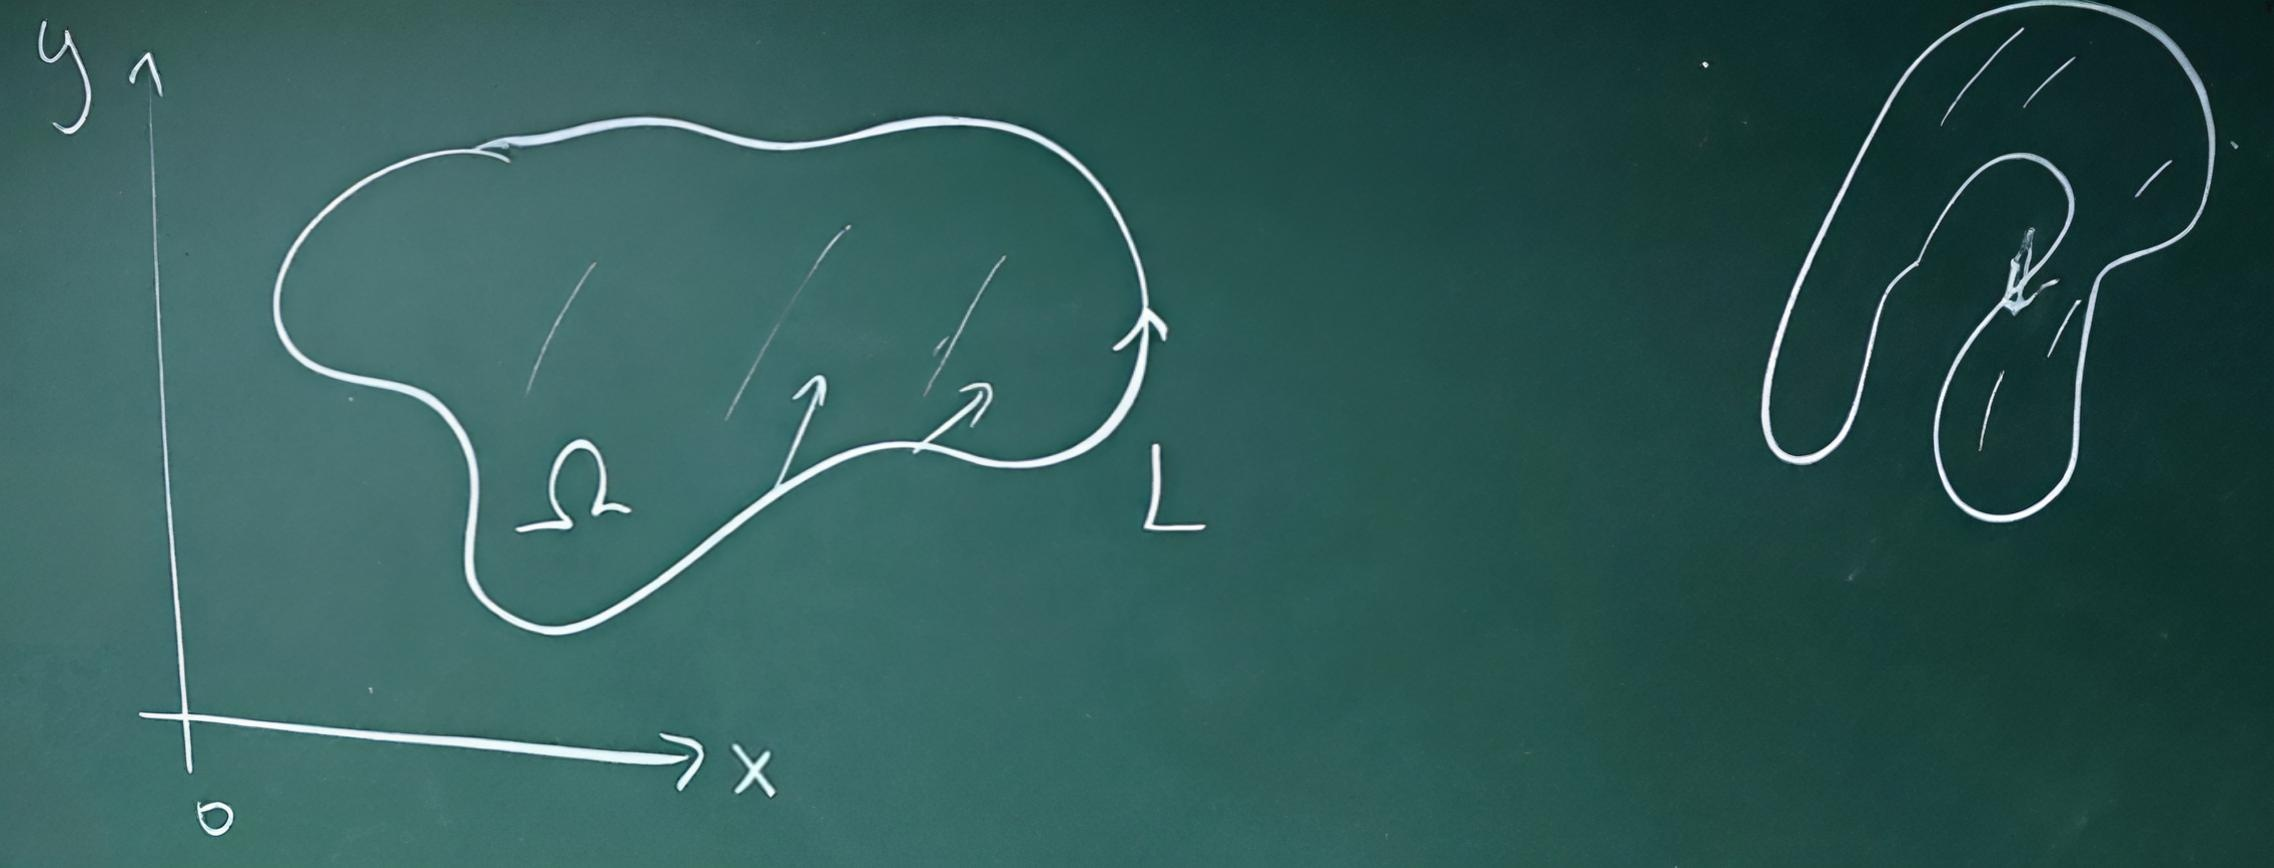
\includegraphics[height=3cm]{chapters/11/05/0001}
\end{center}

$$\oint\limits_{\left(L,O_{\text{Anti}}\right)}\underset{\leadsto\overrightarrow{F}=P\overrightarrow{i}+Q\overrightarrow{j}}{P\,\mathrm{d}x+Q\,\mathrm{d}y}=\iint\limits_{\underset{\substack{\downarrow\\\text{the domain enclosed by }L}}{\Omega}}\left(\frac{\partial Q}{\partial x}-\frac{\partial P}{\partial y}\right)\,\mathrm{d}x\mathrm{d}y$$

\paragraph*{Case 1}

$\Omega=[a,b]\times[c,d]$, $L=\partial\Omega$, $\overrightarrow{F}=P\overrightarrow{i}+Q\overrightarrow{j}$\quad\raisebox{-0.5\height}{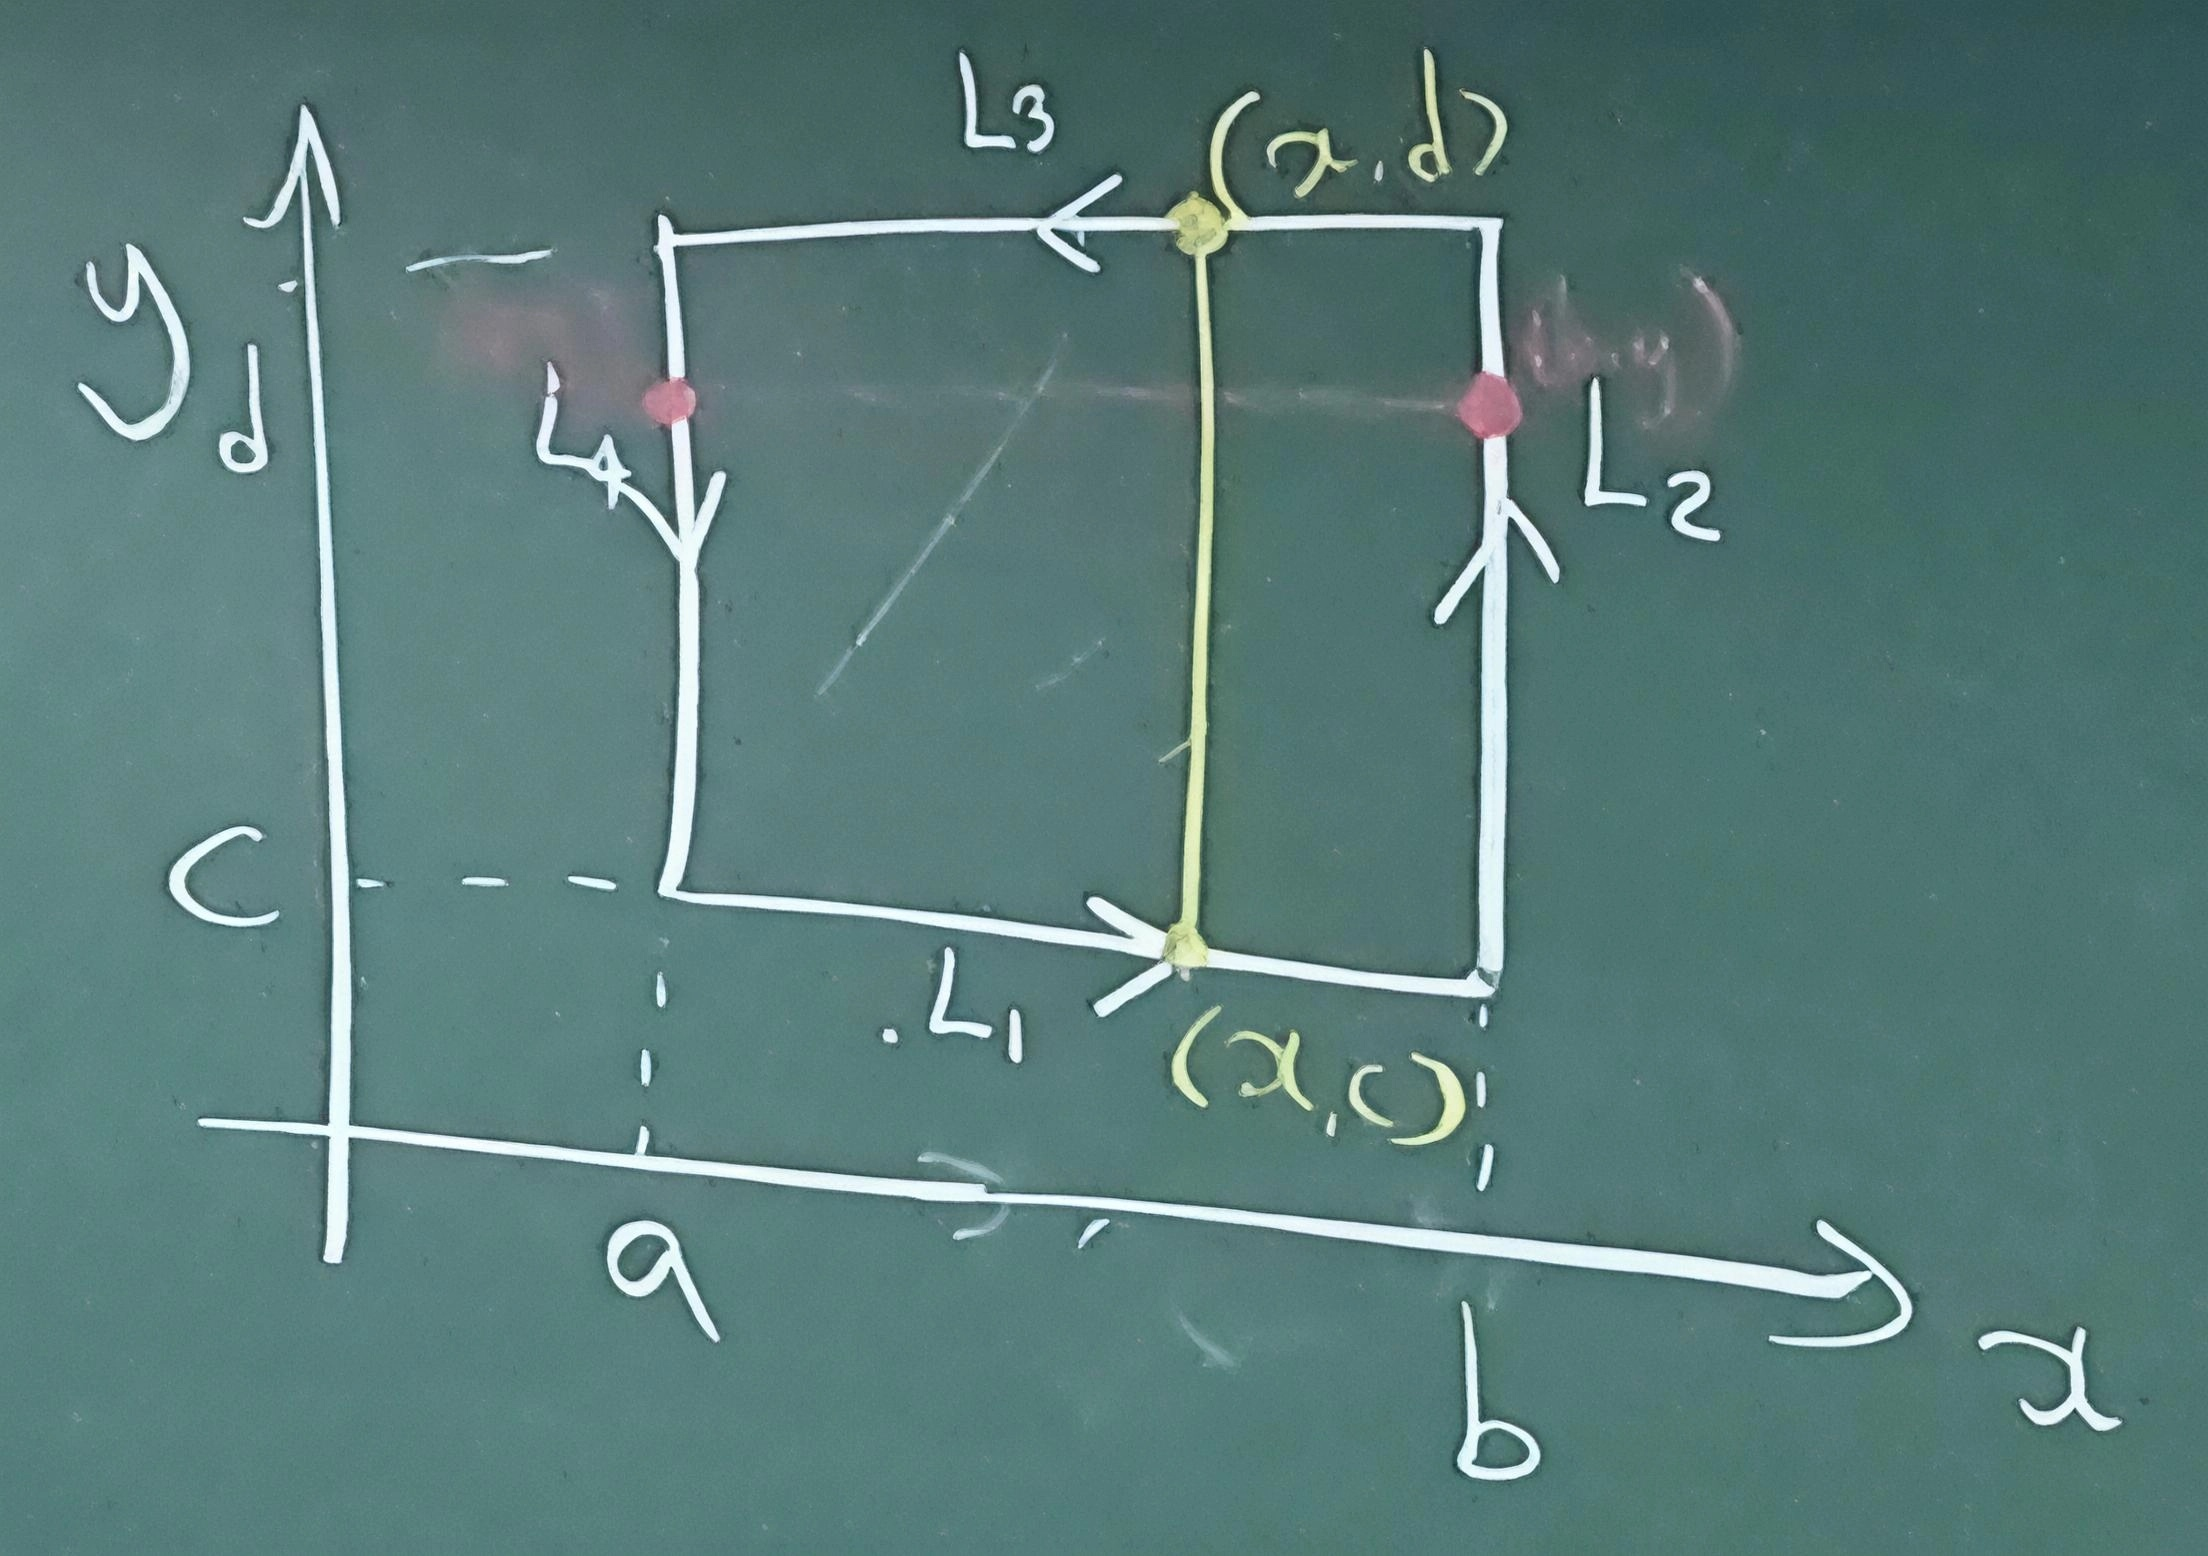
\includegraphics[height=2cm]{chapters/11/05/0002}}

\begin{align*}
    \oint_{\left(L,O_{\text{Anti}}\right)}P\,\mathrm{d}x+Q\,\mathrm{d}y
     & =\int_a^b P(x,c)\,\mathrm{d}x+\int_c^d Q(b,y)\,\mathrm{d}y-\int_a^b P(x,d)\,\mathrm{d}x-\int_c^d Q(a,y)\,\mathrm{d}y                                                                                                     \\
     & =\int_c^d\left(Q(b,y)-Q(a,y)\right)\,\mathrm{d}y-\int_a^b\left(P(x,d)-P(x,c)\right)\,\mathrm{d}x                                                                                                                         \\
     & \xlongequal[\text{formula horizontally}]{\text{Newton-Leibniz}}\int_c^d\,\mathrm{d}y\int_a^b\frac{\partial Q}{\partial x}(x,y)\,\mathrm{d}x-\int_a^b\,\mathrm{d}x\int_c^d\frac{\partial P}{\partial y}(x,y)\,\mathrm{d}y \\
     & =\iint_{\Omega=[a,b]\times[c,d]}\left(\frac{\partial Q}{\partial x}-\frac{\partial P}{\partial y}\right)\,\mathrm{d}x\mathrm{d}y
\end{align*}

Assumption: $\frac{\partial Q}{\partial x}$, $\frac{\partial P}{\partial y}$ are continuous on $Omega$; $P,Q$ are continuous on $\Omega$.

\paragraph*{Case 2}

$\int(P,Q)\cdot\frac{(1,\phi'(x))}{\sqrt{1+\phi'(x)^2}}\,\mathrm{d}s=\int_a^b(P+Q\phi'(x))\,\mathrm{d}x$

\begin{center}
    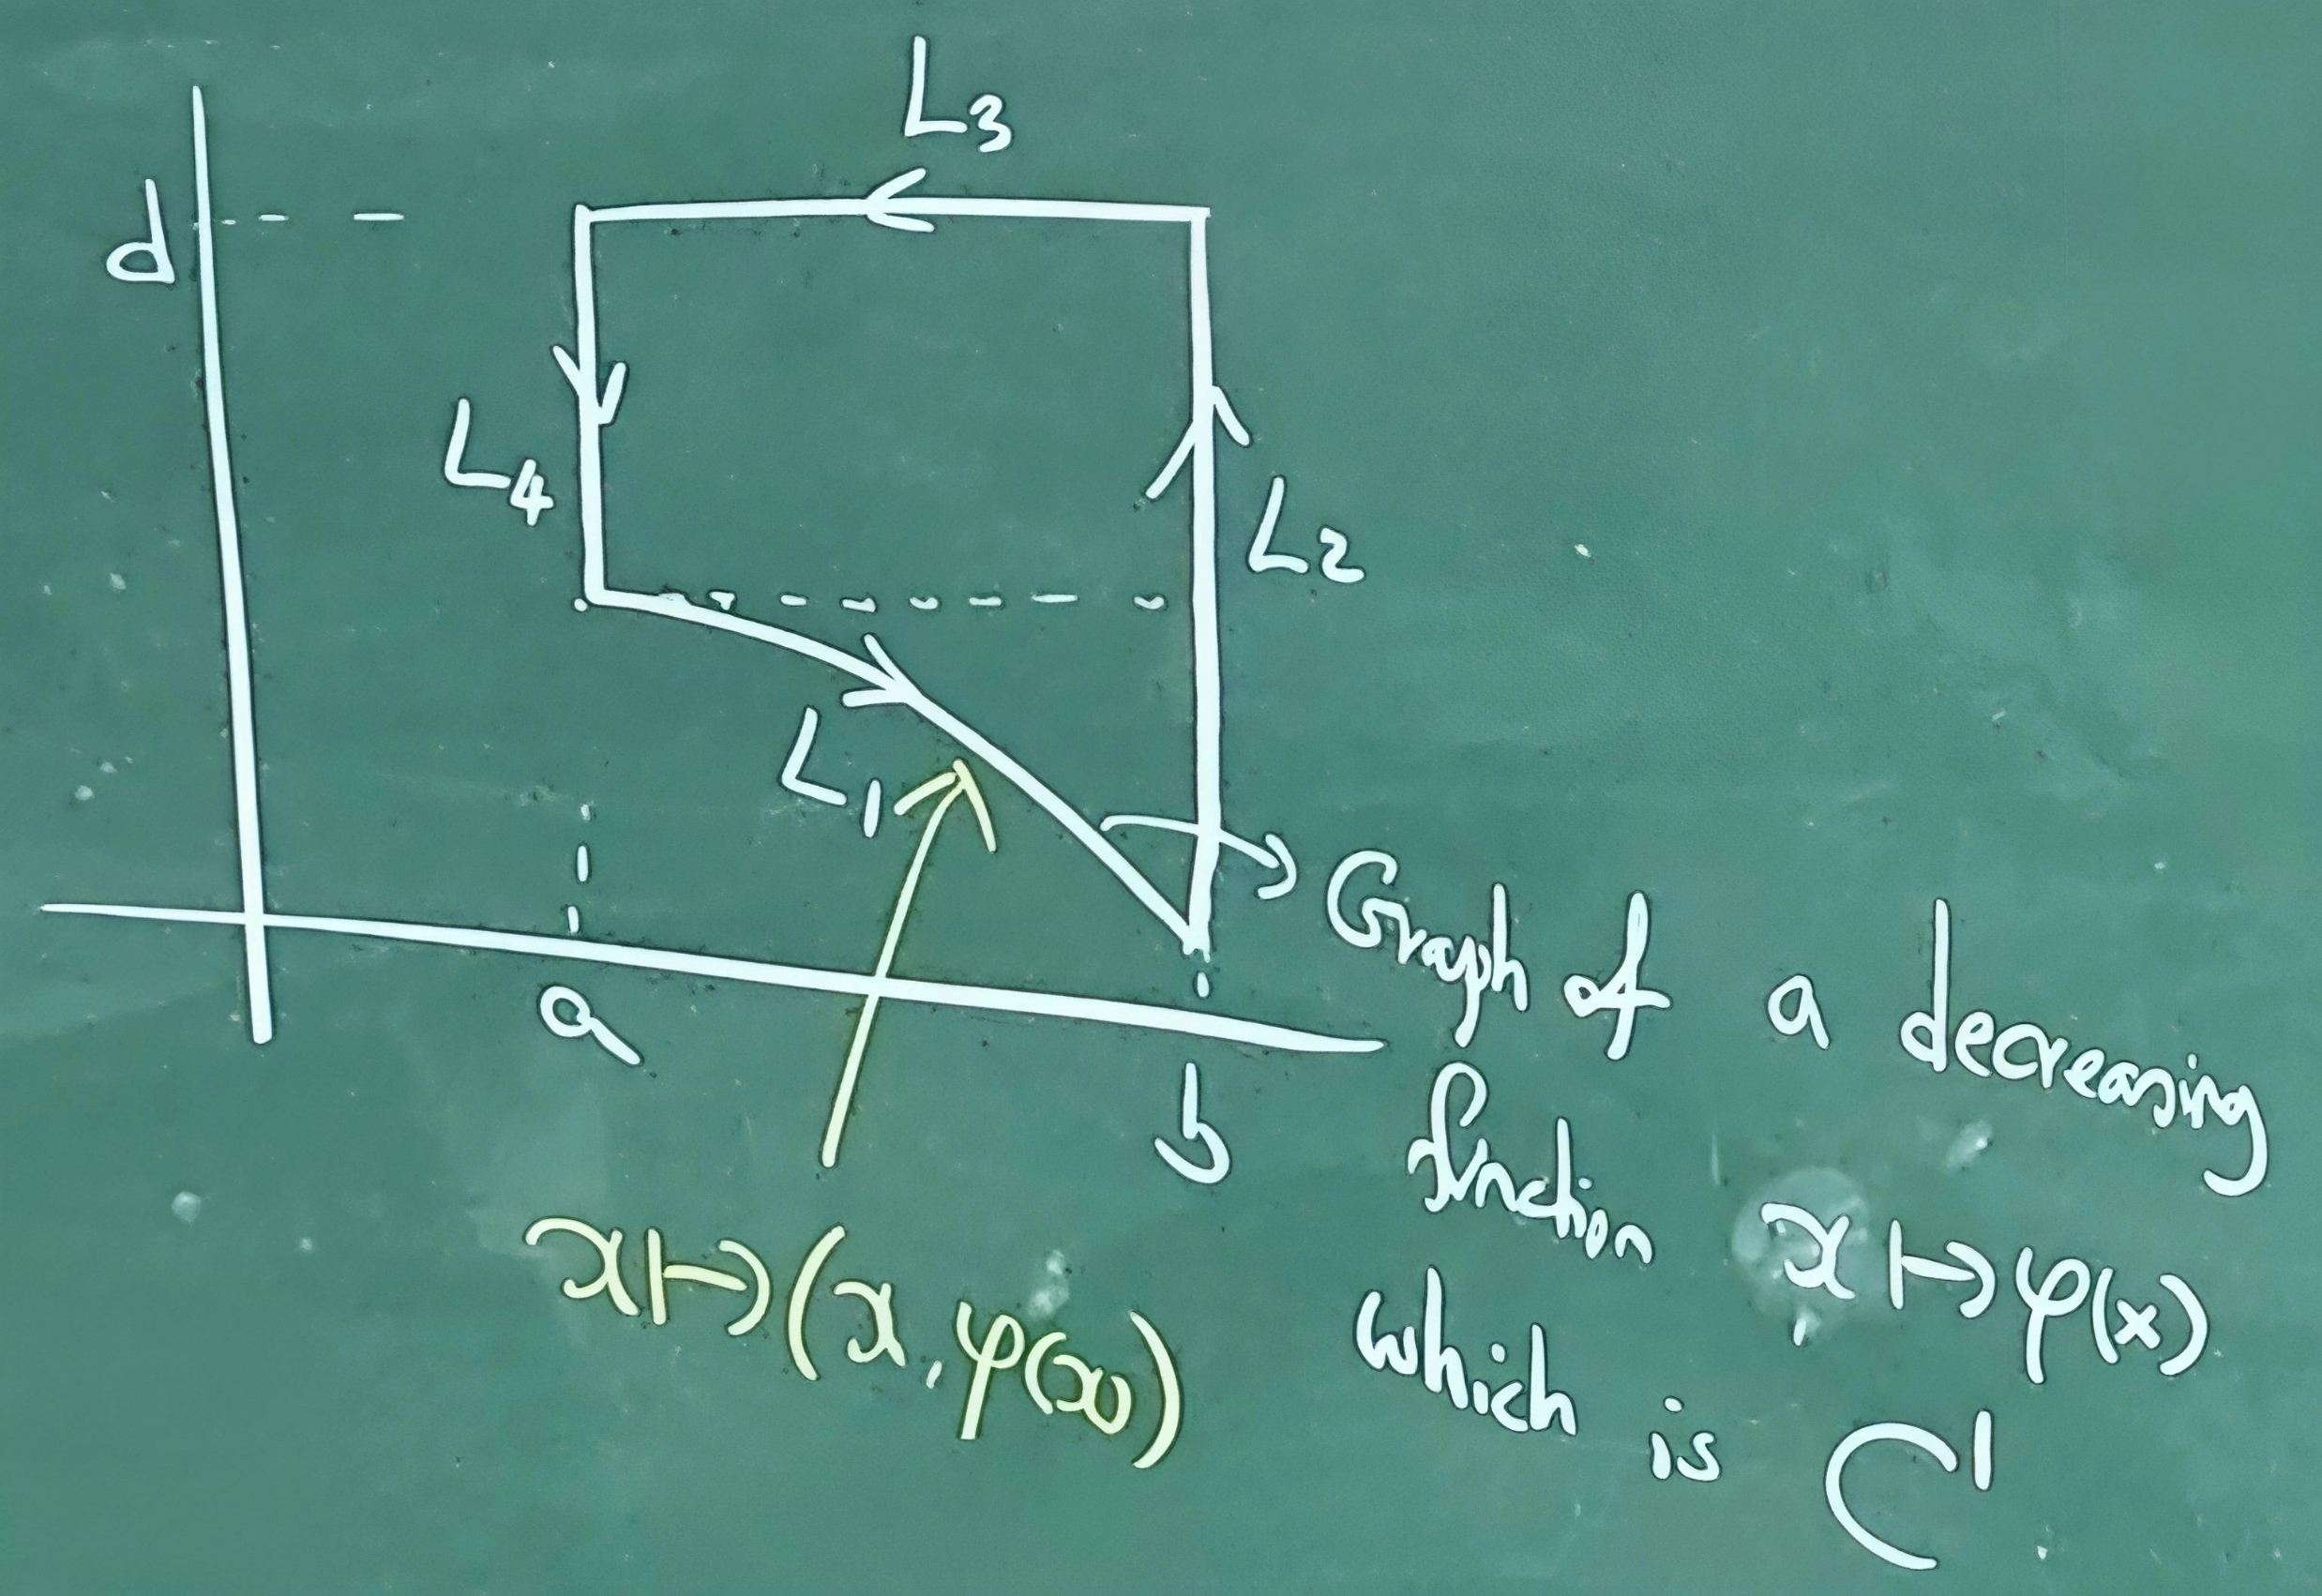
\includegraphics[height=3cm]{chapters/11/05/0003}
\end{center}

\begin{align*}
    \oint_L P\,\mathrm{d}x+Q\,\mathrm{d}y
     & =\int_a^b\left(P(x,\phi(x))+Q(x,\phi(x))\phi'(x)\right)\,\mathrm{d}x                                                                                                        \\
     & \quad+\int_{\phi(b)}^d Q(b,y)\,\mathrm{d}y-\int_a^b P(x,d)\,\mathrm{d}x-\int_{\phi(a)}^d Q(a,y)\,\mathrm{d}y                                                                \\
     & =-\int_a^b\,\mathrm{d}x\int_{\phi(x)}^d\frac{\partial P}{\partial y}(x,y)\,\mathrm{d}y+\int_{\phi(a)}^d\,\mathrm{d}y\int_a^b\frac{\partial Q}{\partial x}(x,y)\,\mathrm{d}x \\
     & \quad+\int_{\phi(b)}^{\phi(a)}Q(b,y)\,\mathrm{d}y+\int_a^b Q(x,\phi(x))\phi'(x)\,\mathrm{d}x                                                                                \\
     & =\iint_{\Omega}\left(\frac{\partial Q}{\partial x}-\frac{\partial P}{\partial y}\right)\,\mathrm{d}x\mathrm{d}y
\end{align*}

\begin{align*}
    \int_{\phi(b)}^{\phi(a)}Q(b,y)\,\mathrm{d}y+\int_a^b Q(x,\phi(x))\phi'(x)\,\mathrm{d}x
     & \xlongequal{y=\phi(x)}\int_{\phi(b)}^{\phi(a)}Q(b,y)\,\mathrm{d}y+\int_{\phi(a)}^{\phi(b)}Q(\phi^{-1}(y),y)\,\mathrm{d}y \\
     & =\int_{\phi(b)}^{\phi(a)}\left(Q(b,y)-Q(\phi^{-1}(y),y)\right)\,\mathrm{d}y                                              \\
     & =\int_{\phi(b)}^{\phi(a)}\,\mathrm{d}y\int_{\phi^{-1}(y)}^b\frac{\partial Q}{\partial x}(x,y)\,\mathrm{d}x               \\
     & =\iint_{\Omega'}\frac{\partial Q}{\partial x}(x,y)\,\mathrm{d}x\mathrm{d}y
\end{align*}

% 20260521

\subparagraph*{Green's Theorem}

Let $D\subseteq\mathbb{R}^2$ be a bounded open set with boundary $\partial D=\sqcup_{k=1}^N L_k$ ($L_1,\dots,L_N$ are ptecewisely $C^1$ curve). Let $\overrightarrow{v}=P(x,y)\overrightarrow{i}+Q(x,y)\overrightarrow{j}$ be a continuous vector field on $\overline{D}$, such that $\frac{\partial P}{\partial y}$, $\frac{\partial Q}{\partial x}$ are also continuous on $\overline{D}$, then

$$
    \oint_{\left(\partial D, O_{\text{Anti}}\right)}\overrightarrow{v}\cdot\mathrm{d}\overrightarrow{r}=\oint_{\partial D}P\,\mathrm{d}x+Q\,\mathrm{d}y=\iint\limits_D\left(\frac{\partial Q}{\partial x}-\frac{\partial P}{\partial y}\right)\,\mathrm{d}x\mathrm{d}y\quad\text{(二重积分)}
$$

\begin{example}
    Consider

    \begin{align*}
        \oint\limits_{\left(\partial D,O_{\text{Anti}}\right)}x\,\mathrm{d}y  & =\iint\limits_D\,\mathrm{d}x\mathrm{d}y=\operatorname{Area}(D)                                   \\
        \oint\limits_{\left(\partial D,O_{\text{Anti}}\right)}-y\,\mathrm{d}x & =\iint\limits_D\,\mathrm{d}x\mathrm{d}y=\operatorname{Area}(D)                                   \\
        \implies\operatorname{Area}(D)                                        & =\frac{1}{2}\oint\limits_{\left(\partial D,O_{\text{Anti}}\right)}-y\,\mathrm{d}x+x\,\mathrm{d}y
    \end{align*}

    \raisebox{-0.5\height}{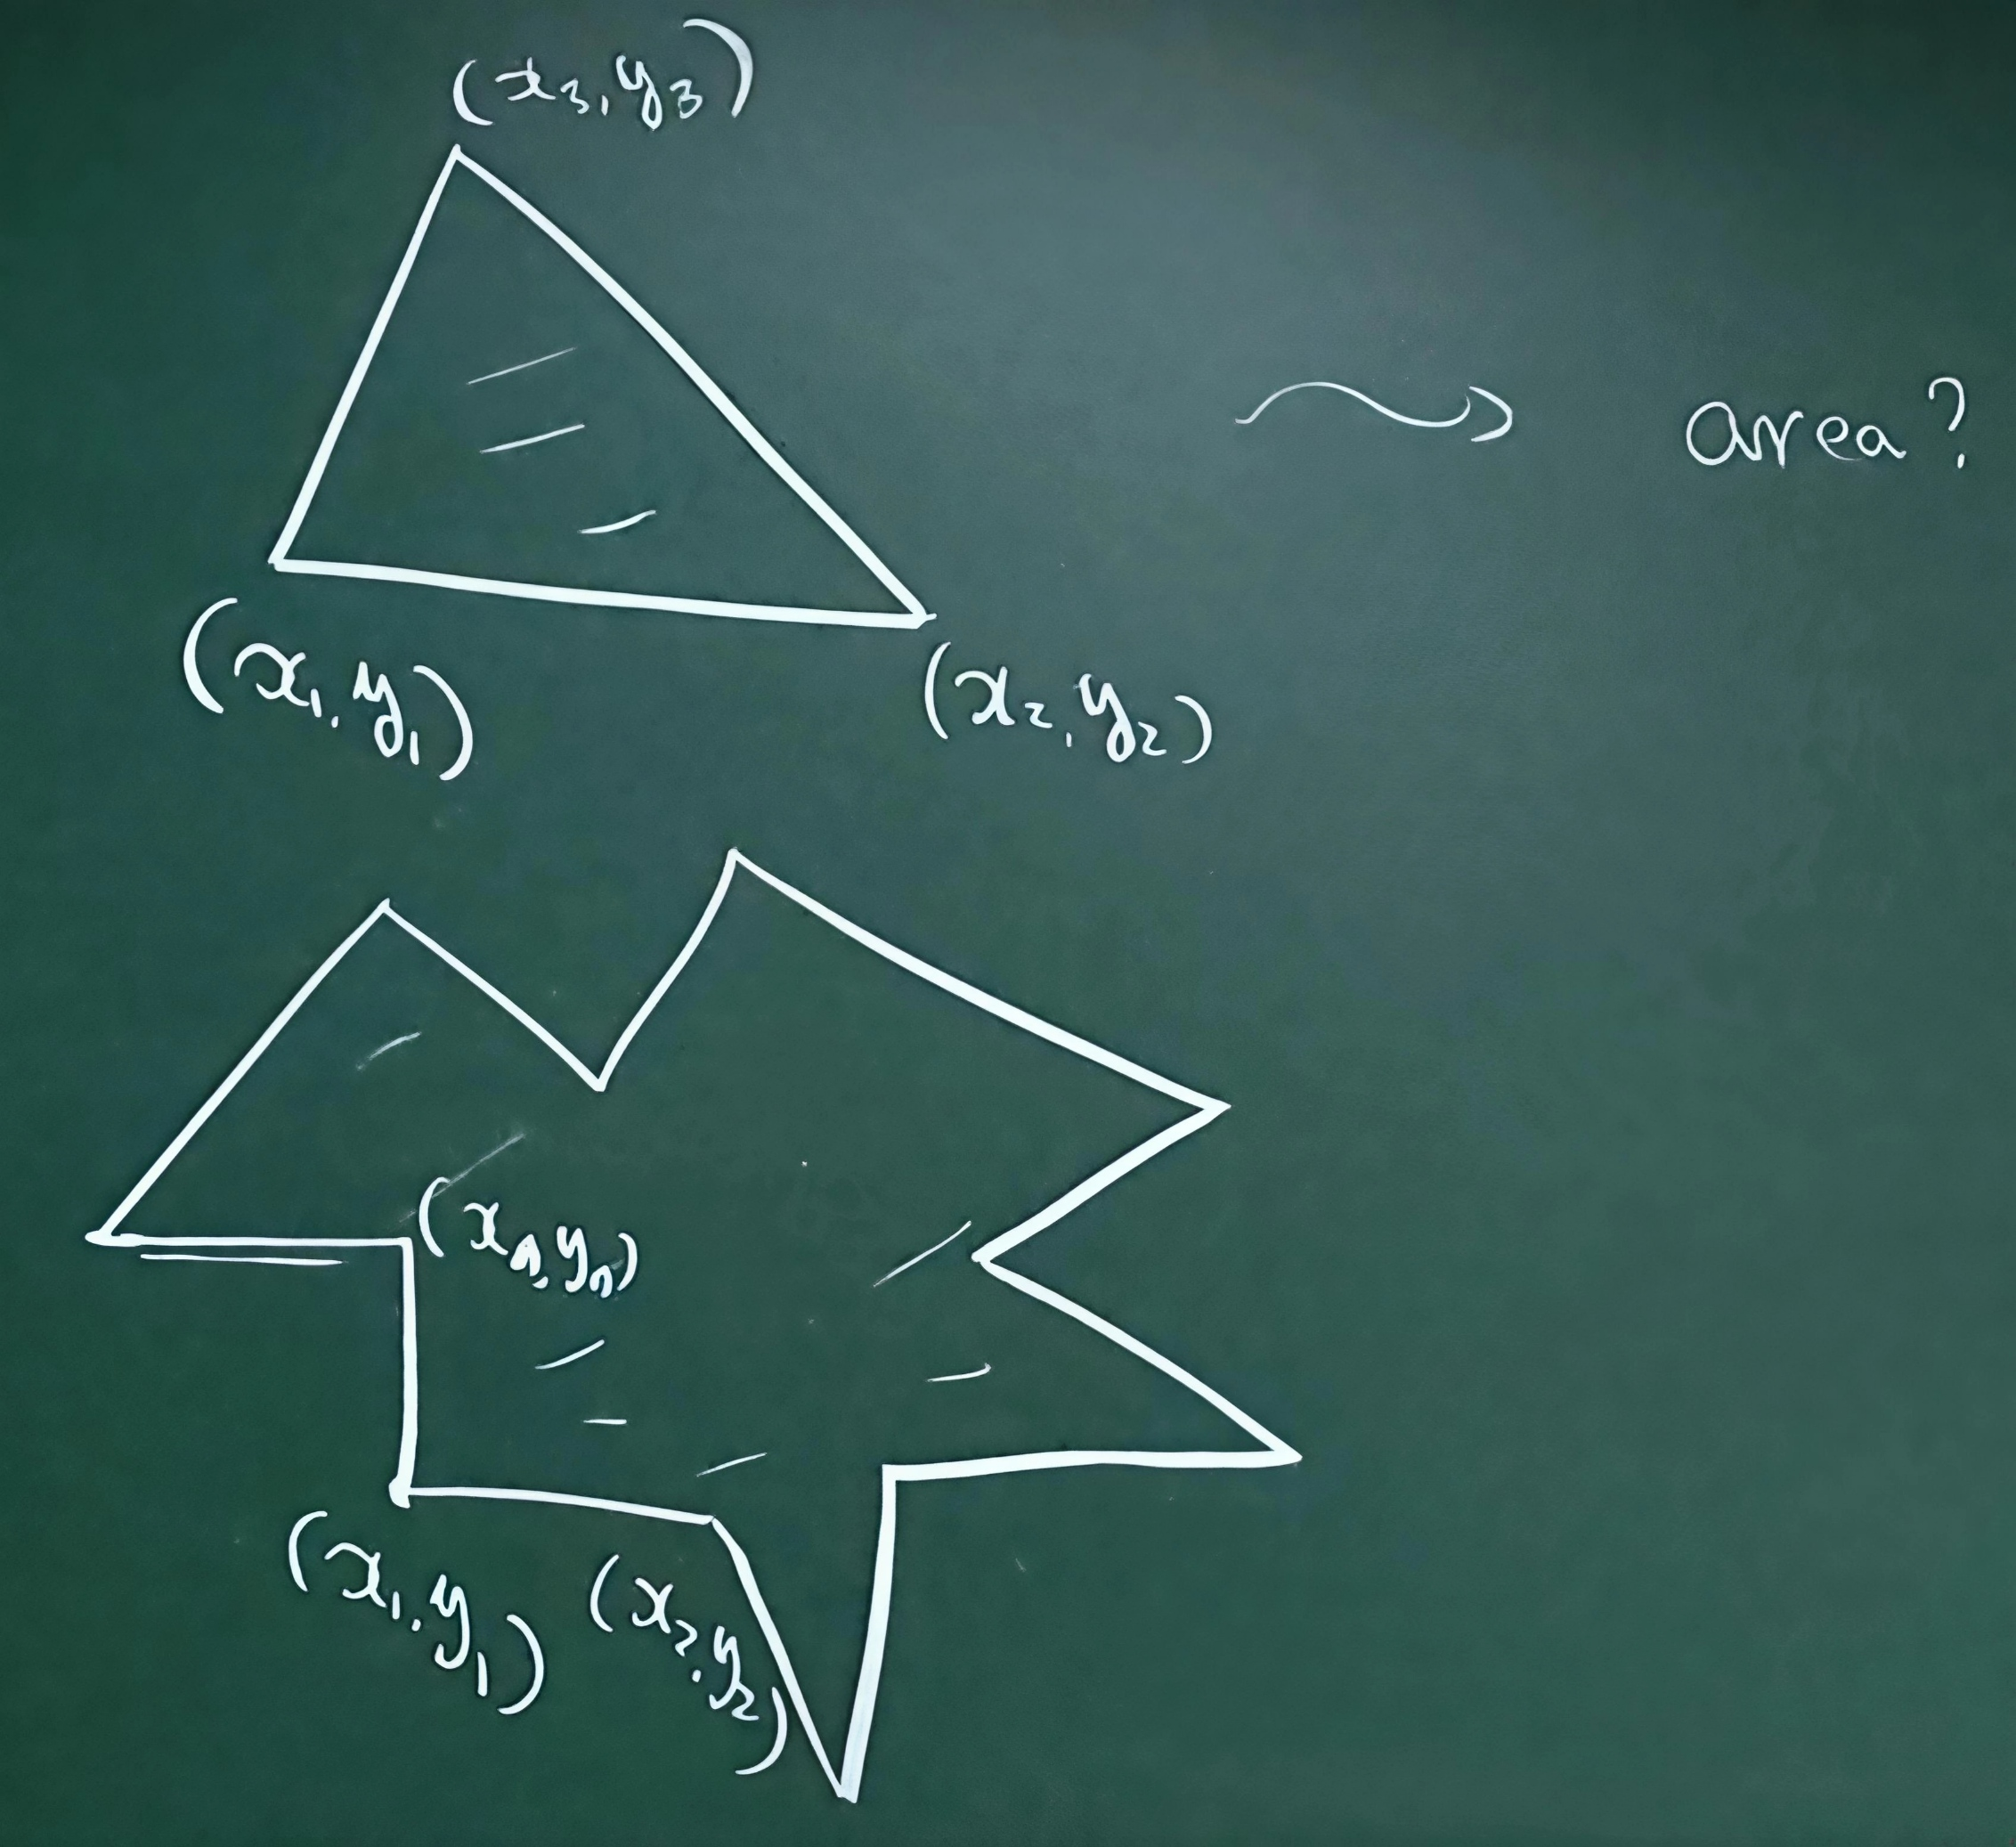
\includegraphics[height=4cm]{chapters/11/05/0004}}\quad$\displaystyle\implies\text{Area}=\frac{1}{2}\sum_{i=1}^n\begin{vmatrix}
            x_i     & y_i     \\
            x_{i+1} & y_{i+1}
        \end{vmatrix}$
\end{example}

On the segment \raisebox{-0.5\height}{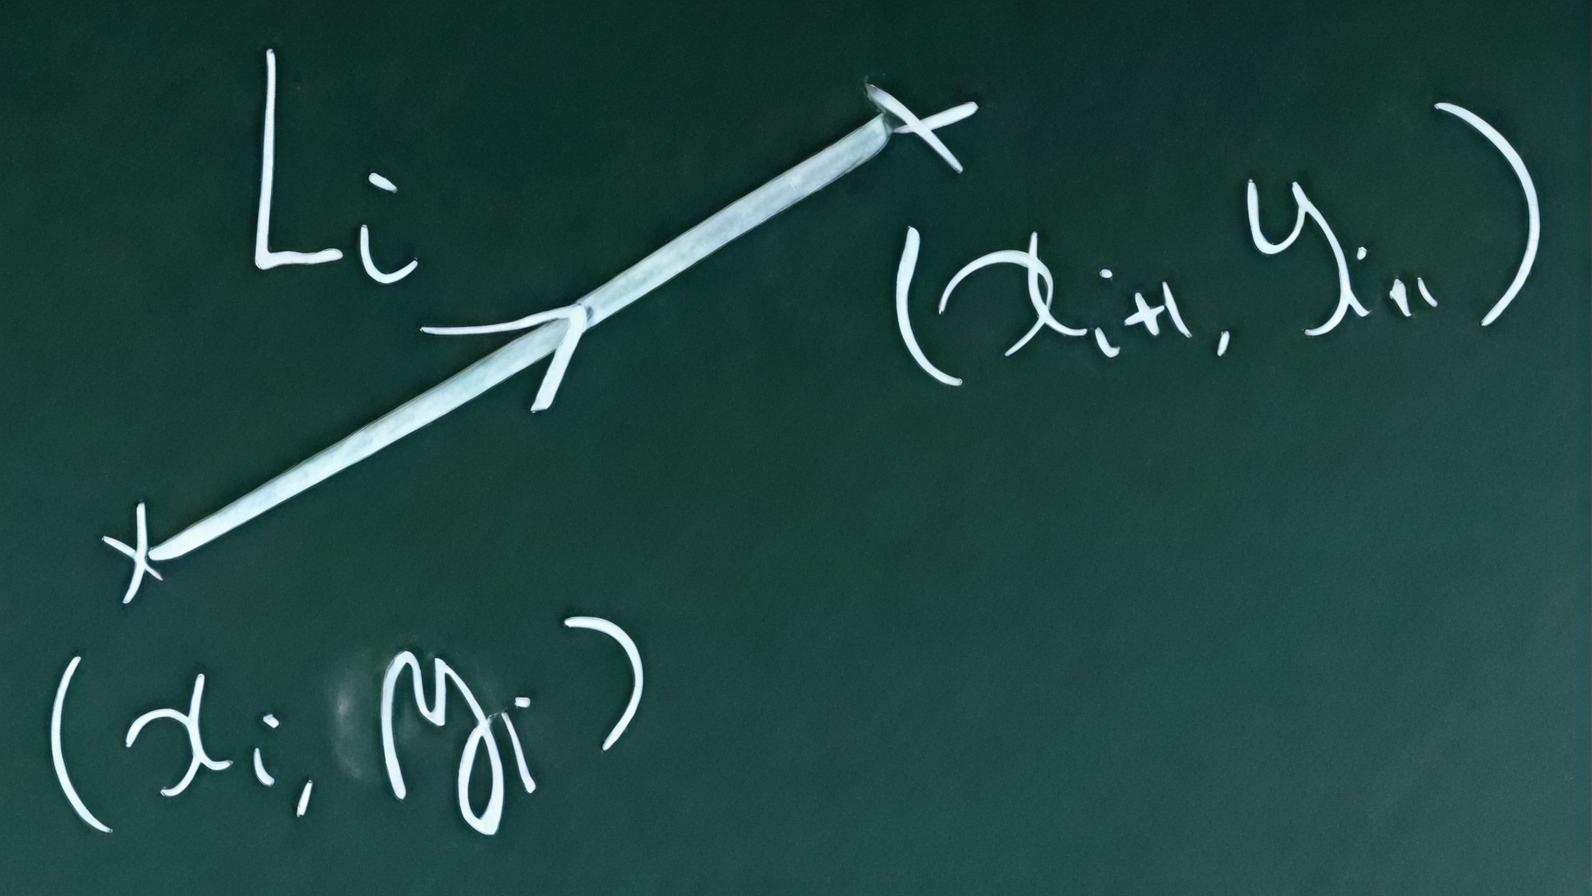
\includegraphics[height=1cm]{chapters/11/05/0005}}, use parametrization
$$t\mapsto(1-t)(x_i,y_i)+t(x_{i+1},y_{i+1})=\left((1-t)x_i+tx_{i+1},(1-t)y_i+ty_{i+1}\right),\quad t\in[0,1]$$
\begin{align*}
    \frac{1}{2}\int_{L_i}-y\,\mathrm{d}x+x\,\mathrm{d}y
     & =\frac{1}{2}\int_0^1\left\{-\left((1-t)y_i+ty_{i+1}\right)(x_{i+1}-x_i)+\left((1-t)x_i+tx_{i+1}\right)(y_{i+1}-y_i)\right\}\,\mathrm{d}t \\
     & =\frac{1}{2}\int_0^1\left\{(1-t)(x_iy_{i+1}-x_{i+1}y_i)+t\left(x_{i+1}(y_{i+1}-y_i)-y_{i+1}(x_{i+1}-x_i)\right)\right\}\,\mathrm{d}t     \\
     & =\frac{1}{2}\begin{vmatrix}
                       x_i     & y_i     \\
                       x_{i+1} & y_{i+1}
                   \end{vmatrix}
\end{align*}

\begin{example}
    Let $L$ be a simple closed $C^1$ curve around $(0,0)$, with anti-clockwise orientation. Compute $\oint_L\frac{-y\,\mathrm{d}x+x\,\mathrm{d}y}{x^2+y^2}$

    Take $\varepsilon>0$ sufficiently small, let $D$ be the domain enclosed by $L$.

    \begin{align*}
        \oint\limits_{\left(\partial\left(D\setminus B(0,\varepsilon)\right),O_{\text{Anti}}\right)}\frac{-y\,\mathrm{d}x+x\,\mathrm{d}y}{x^2+y^2}
         & =\oint\limits_{\left(L,O_{\text{Anti}}\right)}\frac{-y\,\mathrm{d}x+x\,\mathrm{d}y}{x^2+y^2}-\oint\limits_{\left(\partial B(0,\varepsilon),O_{\text{Anti}}\right)}\frac{-y\,\mathrm{d}x+x\,\mathrm{d}y}{x^2+y^2} \\
         & \xlongequal{\text{Green's Thm}}\iint\limits_{D\setminus B(0,\varepsilon)}\left(\frac{\partial}{\partial x}\frac{x}{x^2+y^2}-\frac{\partial}{\partial y}\frac{-y}{x^2+y^2}\right)\,\mathrm{d}x\mathrm{d}y         \\
         & =0
    \end{align*}

    \begin{align*}
        \implies\oint\limits_{\left(L,O_{\text{Anti}}\right)}\frac{-y\,\mathrm{d}x+x\,\mathrm{d}y}{x^2+y^2}
         & \xlongequal[\text{sufficiently small}]{\text{for any fixed $\varepsilon>0$}}\oint\limits_{\left(\partial B(0,\varepsilon),O_{\text{Anti}}\right)}\frac{-y\,\mathrm{d}x+x\,\mathrm{d}y}{x^2+y^2} \\
         & \xlongequal[{\theta\in\left[0,2\pi\right]}]{\substack{x=\varepsilon\cos\theta                                                                                                                   \\y=\varepsilon\sin\theta}}\int_0^{2\pi}\frac{-\varepsilon\sin\theta(-\varepsilon\sin\theta)\,\mathrm{d}\theta+\varepsilon\cos\theta(\varepsilon\cos\theta\,\mathrm{d}\theta)}{\varepsilon^2}\\
         & =2\pi
    \end{align*}

    $\rightarrow\overrightarrow{v}=\left(-\frac{y}{x^2+y^2},\frac{x}{x^2+y^2}\right)$
\end{example}

\subparagraph*{Green's Formula}

$\overrightarrow{n}=(n_1,n_2)$ unit outer normal, $u,v$ are $C^2$ function

\begin{align*}
    \implies\oint_{\partial D}v\cdot\frac{\partial u}{\partial\overrightarrow{n}}\,\mathrm{d}s
     & =\iint\limits_D\left(v\Delta u+\nabla u\cdot\nabla v\right)\,\mathrm{d}x\mathrm{d}y \\
    \oint_{\partial D}\left(u\frac{\partial v}{\partial\overrightarrow{n}}-v\frac{\partial u}{\partial\overrightarrow{n}}\right)\,\mathrm{d}s
     & =\iint\limits_D\left(u\Delta v-v\Delta u\right)\,\mathrm{d}x\mathrm{d}y
\end{align*}

$\frac{\partial u}{\partial\overrightarrow{n}}=\nabla u\cdot\overrightarrow{n}$

\begin{align*}
    v\frac{\partial u}{\partial\overrightarrow{n}}\,\mathrm{d}s
     & =v\nabla u\cdot\overrightarrow{n}\,\mathrm{d}s                                            \\
     & =v(u_x,u_y)\cdot(n_1,n_2)\,\mathrm{d}s                                                    \\
     & =v(-u_y,u_x)\cdot\underset{\mathrm{d}\overrightarrow{r}}{\boxed{(-n_2,n_1)\,\mathrm{d}s}} \\
\end{align*}

